\subsection{Histogram computation}
\label{sec:histogram}

\pavol{motivate query; expand with examples}
A histogram succinctly and meaningfully summarizes the data by calculating its distribution, making it a
common analysis task. In this section, we study bit streams that aim to reproduce the most accurate
histogram possible at any bit rate.

\pavol{discuss error metrics and why we chose the histogram intersection}
It is necessary to first define a criteria to compare two
histograms. There are several options and we explored two of them: Earth Mover's Distance~\cite{emd1998} and
histogram intersection~\cite{histogram_intersection1991}. The Earth Mover's Distance represents
the smallest possible amount of work needed to morph one histogram to another. The work is defined as the
amount of change ($y$-axis) times the distance ($x$-axis). The histogram intersection simply computes for each
bin how much it matches the other histogram's bin and does not consider the distance between bins in domain.
We choose histogram intersection because we consider the bin mismatch to be more important than a transform between two histograms.

\pavol{explain results in the curve plots}
With the error metric defined, \Cref{alg:signature} computes a
\emph{histogram-optimized} stream, given an input data set. To understand the characteristics of an
\emph{histogram-optimized} stream that make it suitable for histogram computation, we compare it
with the \emph{rmse-optimized} stream for the same data set. We also include their corresponding
data-independent analouges, namely \emph{histogram signature} and \emph{by wavelet norm} (the
concept of a signature is defined in Section [REF]). Figures \ref{fig:histogram-stream-comparison}
are plots of the EMD errors for these streams on four data sets.



\begin{figure}[h]
	\centering
	\subcaptionbox{\emph{boiler}, 64 bins}
	{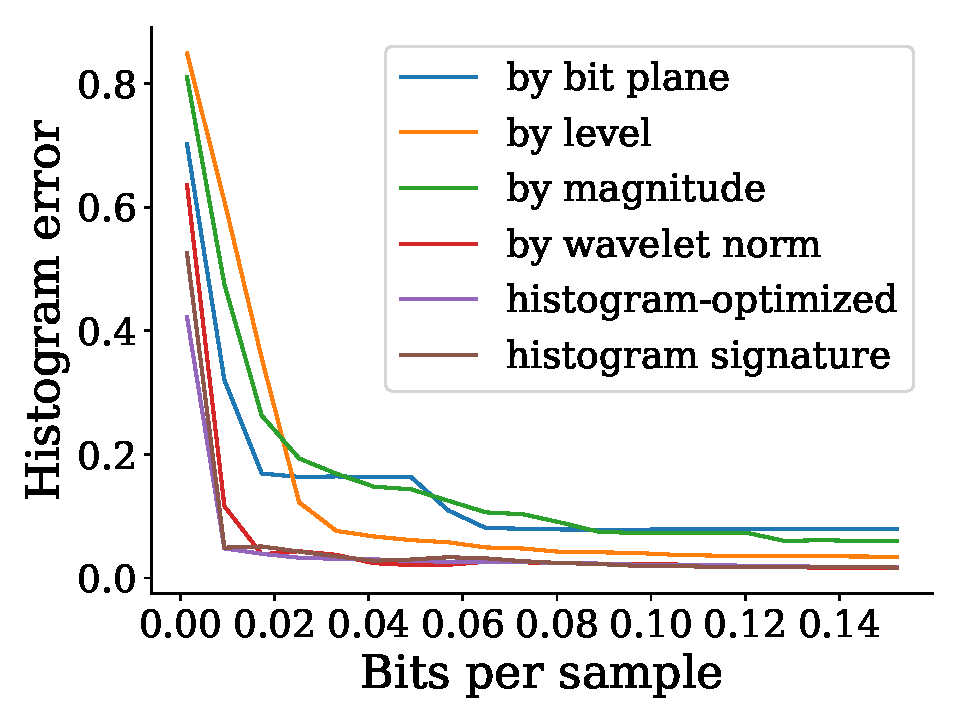
\includegraphics[width=0.48\linewidth]{histogram/histogram-optimized-boiler}}
	\subcaptionbox{\emph{diffusivity}, 64 bins}
	{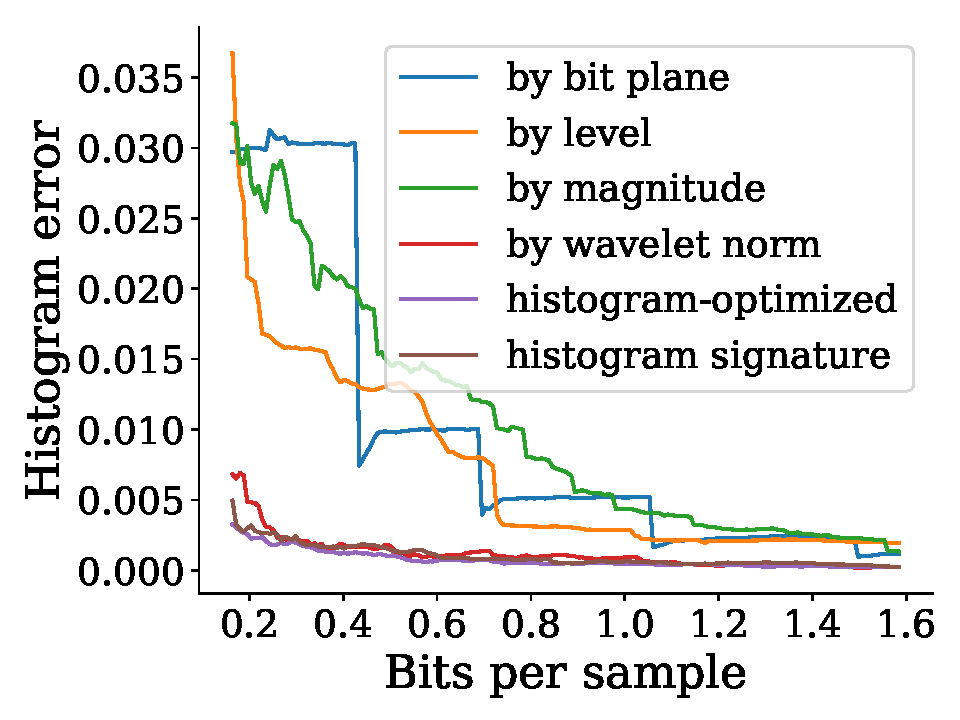
\includegraphics[width=0.48\linewidth]{histogram/histogram-optimized-diffusivity}}
	\subcaptionbox{\emph{plasma}, 64 bins}
	{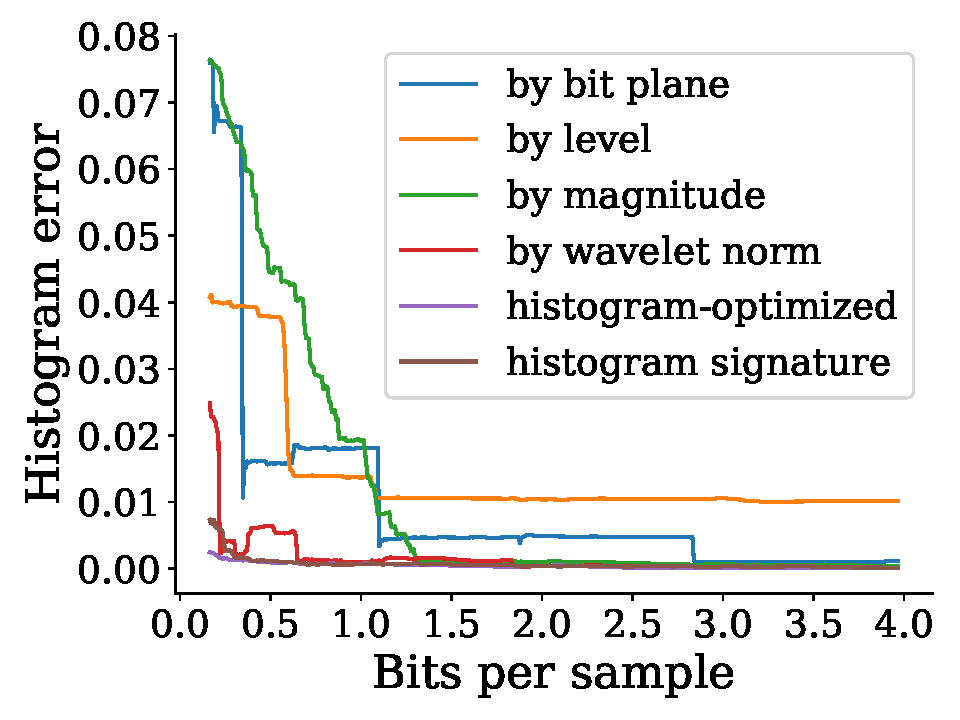
\includegraphics[width=0.48\linewidth]{histogram/histogram-optimized-plasma}}
	\subcaptionbox{\emph{turbulence}, 64 bins}
	{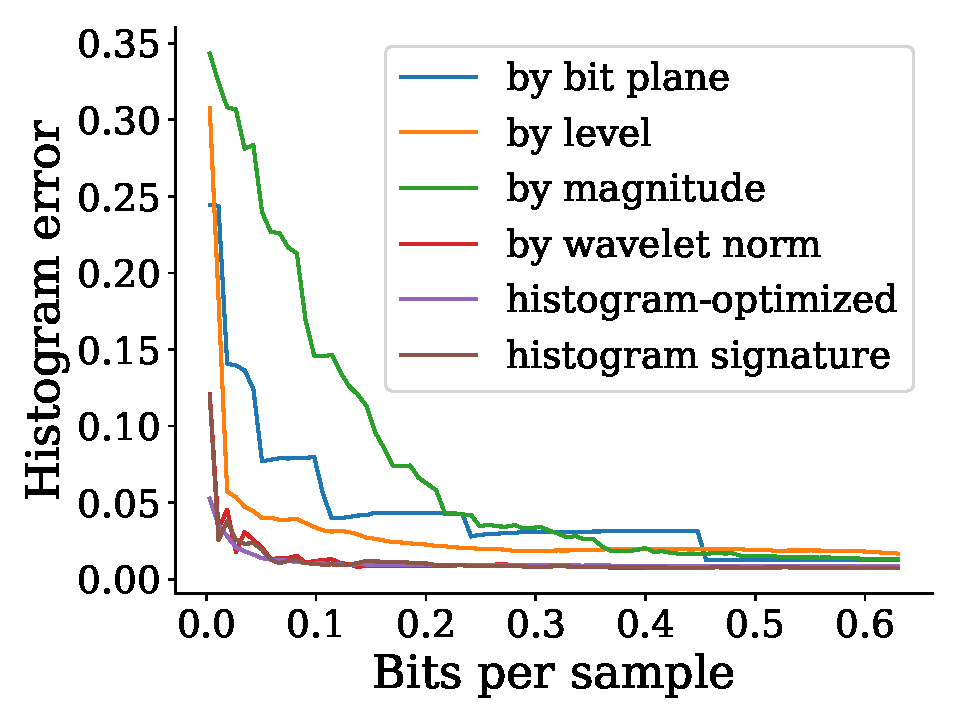
\includegraphics[width=0.48\linewidth]{histogram/histogram-optimized-turbulence}}
	\caption{Histogram error comparison among four streams \emph{histogram-optimized},
	\emph{rmse-optimized}, \emph{by wavelet norm}, and \emph{histogram signature}, without the leading
	zero bits. The plots are truncated to make the differences large enough for visual inspection, and
	truncation points are chosen so that the best among the reconstructed histograms is visually the
	same as the groundtruth histogram. }
	\label{fig:histogram-stream-comparison}
\end{figure}

First, compared to \emph{rmse-optimized}, the \emph{histogram-optimized} stream produces
consistently better histograms. Second, between the two data-independent streams, \emph{histogram
signature} outperforms \emph{by wavelet norm}. To better understand how the Earth mover's distance
translates to visual differences, we visualize the histograms produced by the different streams, at
low bit rates, in Figure \ref{fig:histogram-comparison-low-bit-rate}. These plots confirm our
observations.
\emph{histogram-optimized} and \emph{histogram signature}
outperform \emph{rmse-optimized} and \emph{by wavelet norm} respectively. For example, Figure
\ref{fig:histogram-comparison-low-bit-rate-slz} shows the four reconstructed histograms at 0.1 bits
per sample, with leading zero bits removed, for the diffusivity data set.

\pavol{explain visual results}
Additionally to computing the error curves, we explored several bit rates after the curves exhibit
reasonable error and the histograms are not wildy different from the groundtruth. For example, the {\em boiler}
data set's histogram for each streams confirms the results from the error curves~(\Cref{fig:histograms-boiler}).
The {\em by bit plane} stream or the {\em by magnitude} stream has vastly different shape and scale than the other
streams. The primary cause is that histograms require precision more than resolution, and since these streams\pavol{todo: by magnitude}
always load full resolution but at limited precision, they spent large portion of the bit budget on the resolution part.

\begin{figure}[h]
	\centering
	\subcaptionbox{\emph{by level}}{
	{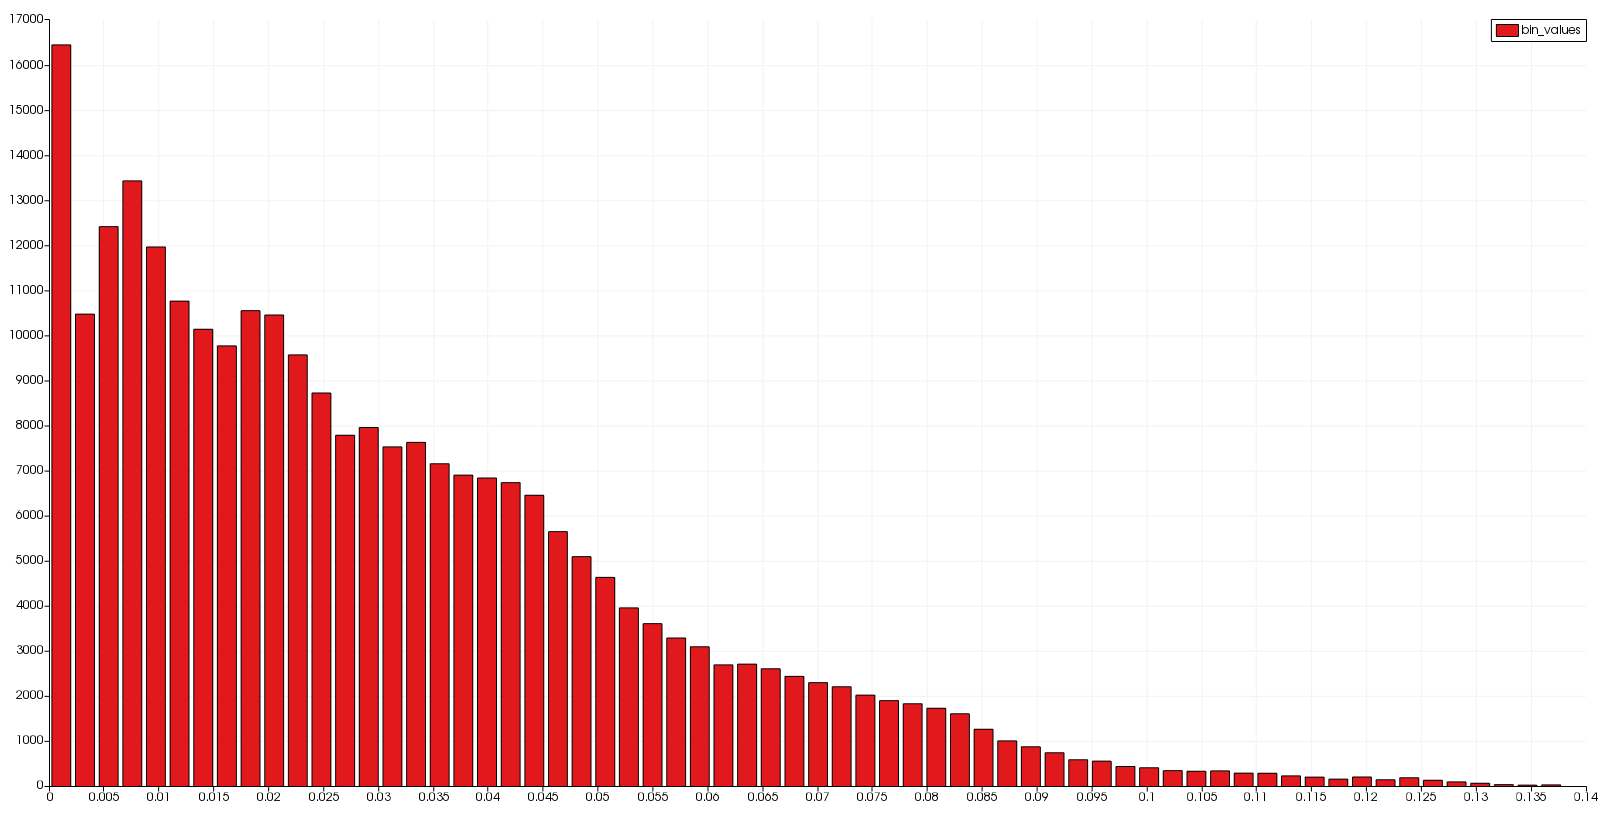
\includegraphics[width=0.31\linewidth]{histogram/histogram-boiler-level.png}}}
	\subcaptionbox{\emph{by bit plane}}{
	{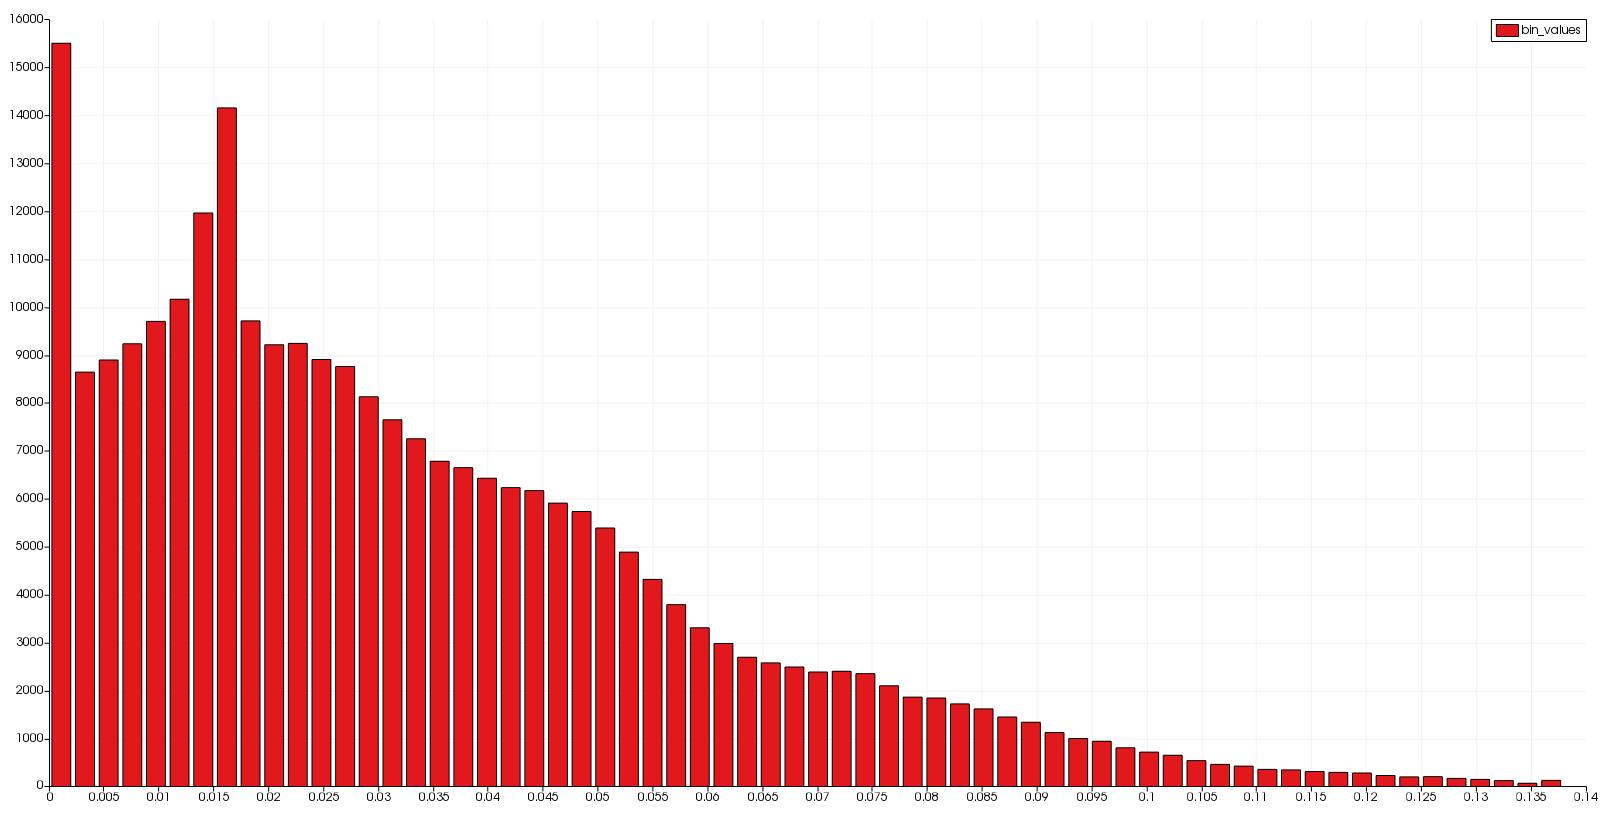
\includegraphics[width=0.31\linewidth]{histogram/histogram-boiler-bit-plane.png}}}
	\subcaptionbox{\emph{by magnitude}}{
	{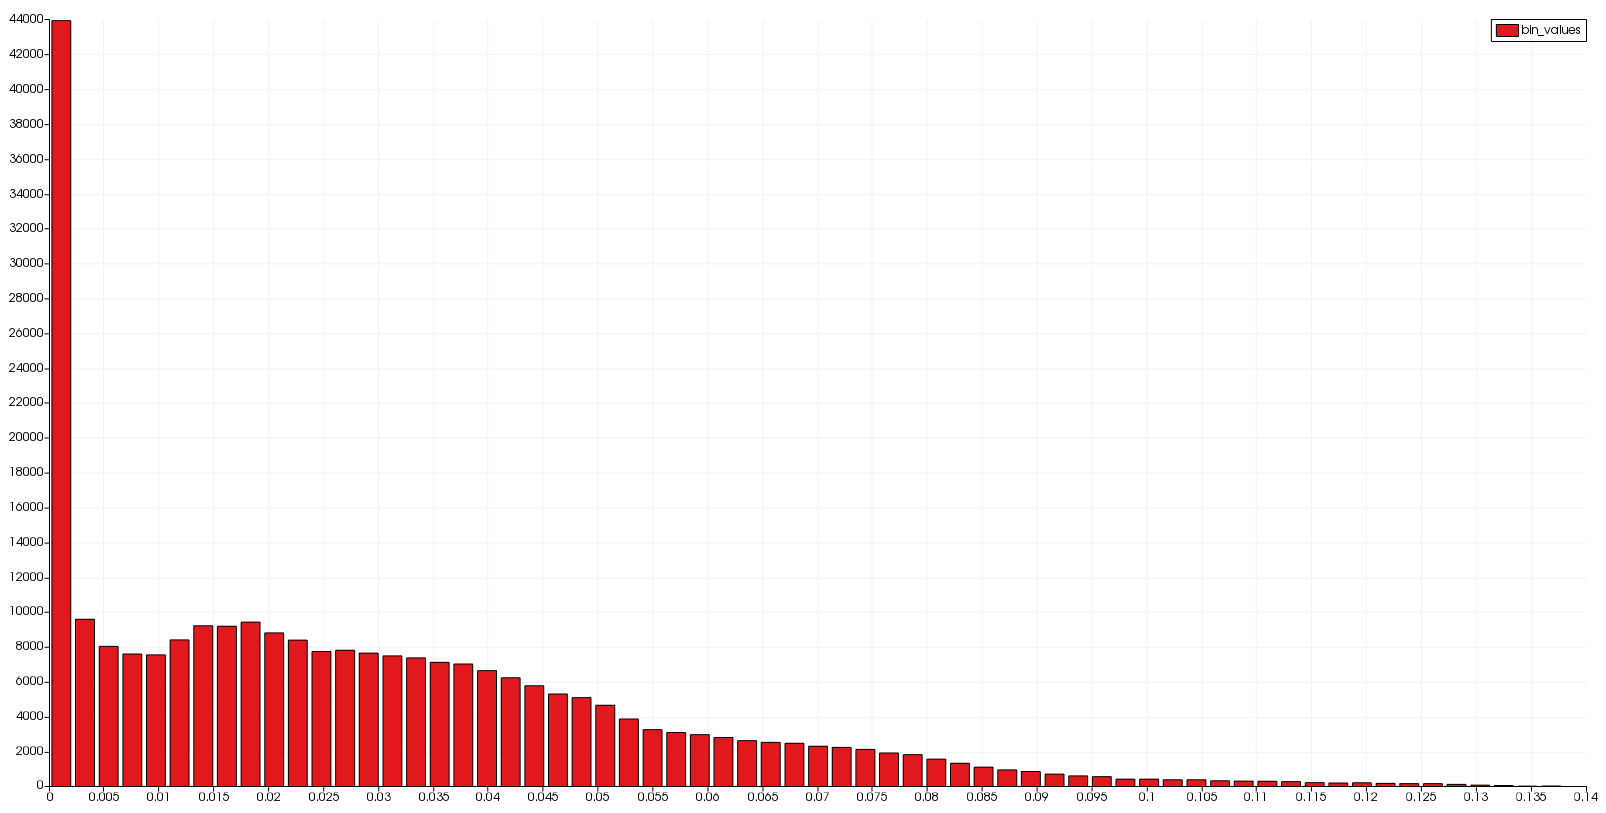
\includegraphics[width=0.31\linewidth]{histogram/histogram-boiler-magnitude.png}}}
	\subcaptionbox{\emph{by wavelet norm}}{
	{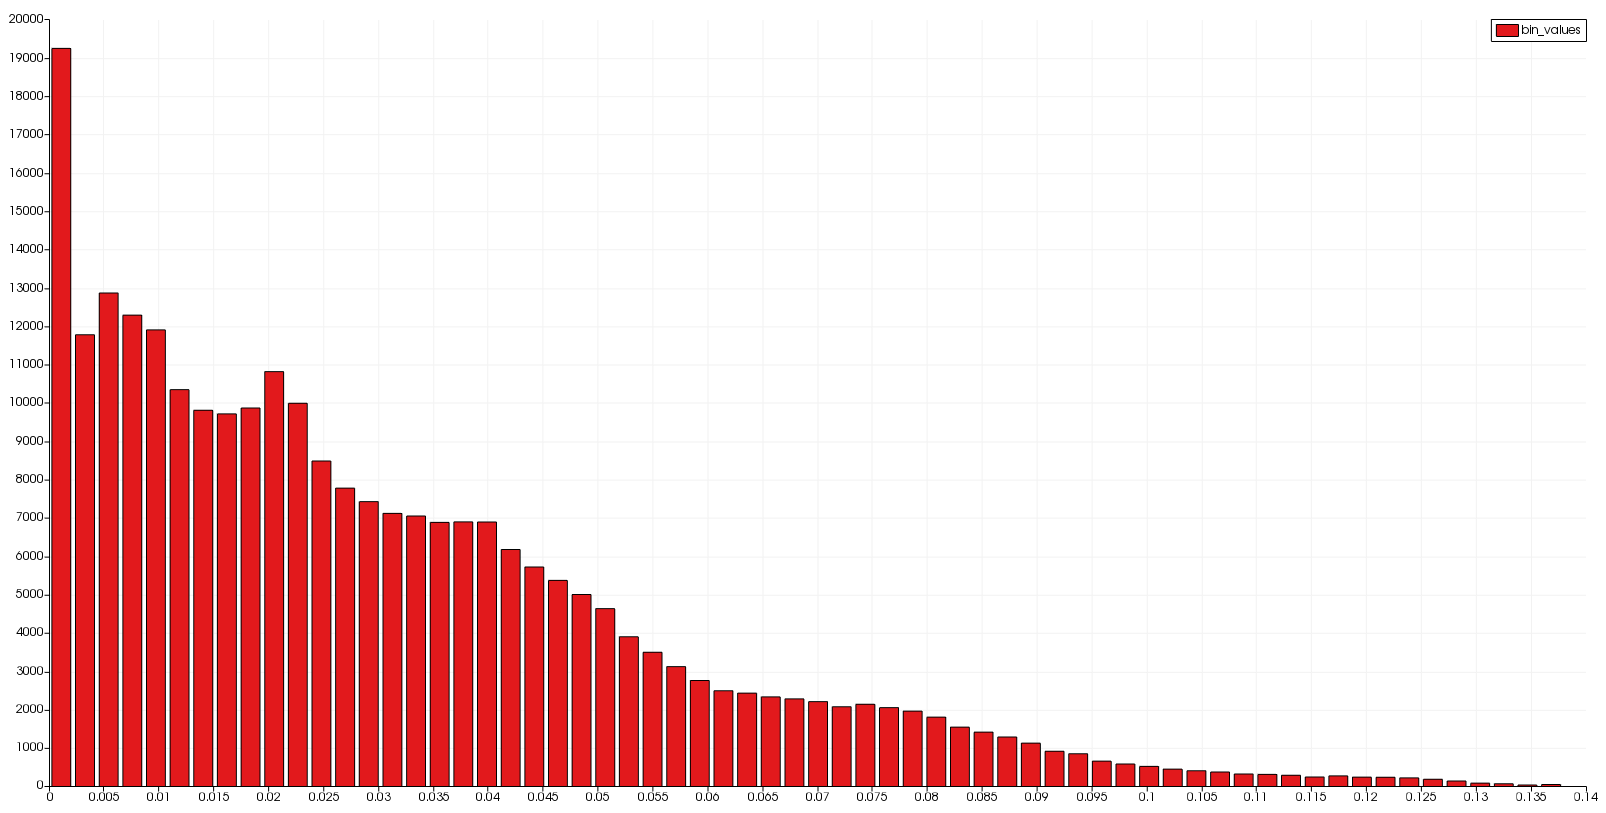
\includegraphics[width=0.31\linewidth]{histogram/histogram-boiler-wavelet-norm.png}}}
	\subcaptionbox{\emph{by signature}}{
	{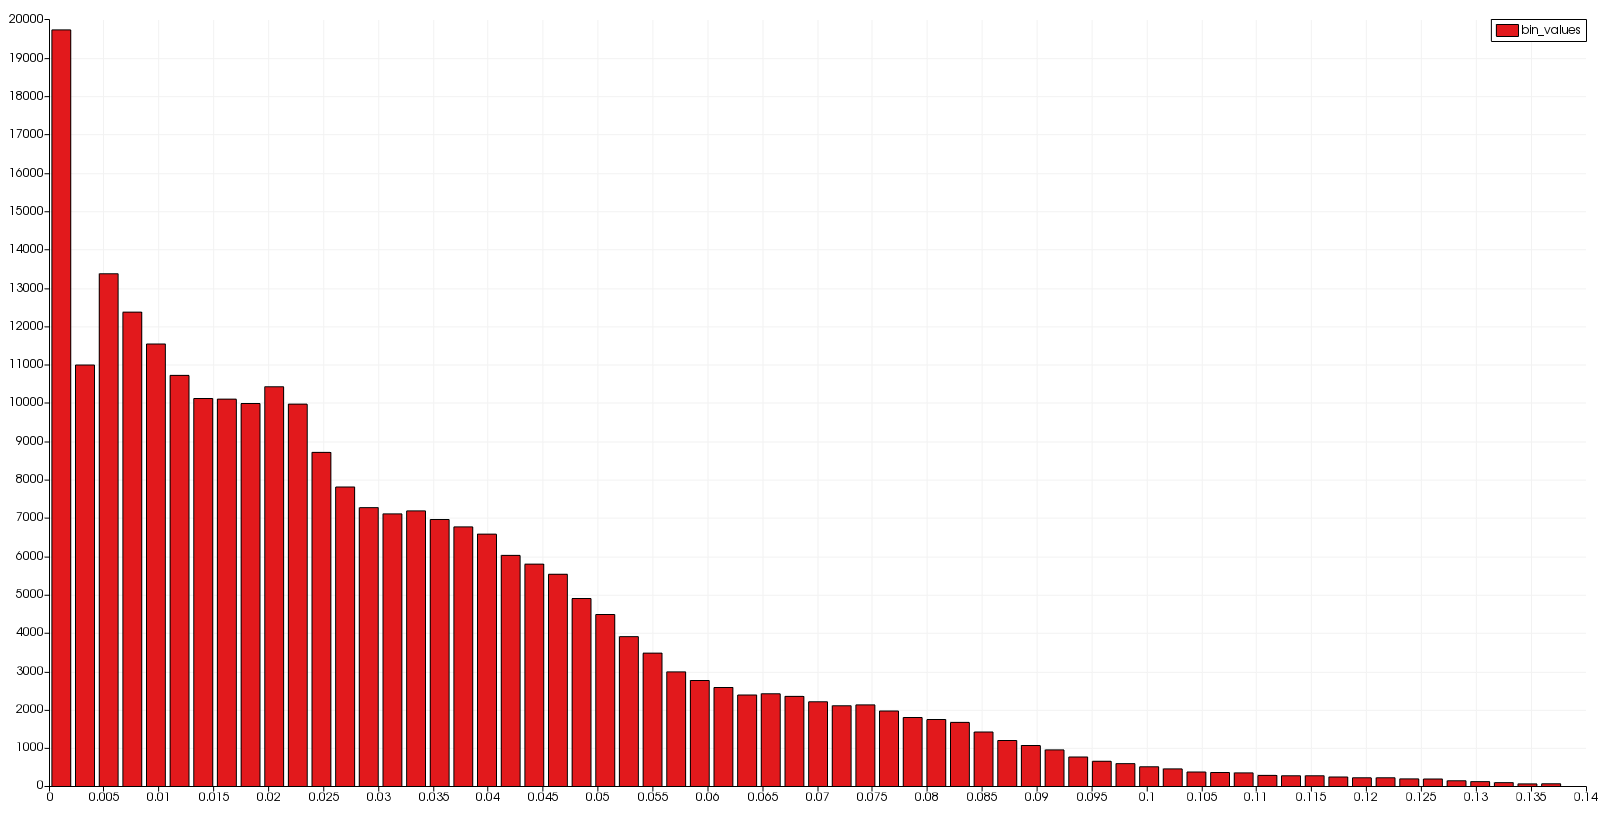
\includegraphics[width=0.31\linewidth]{histogram/histogram-boiler-signature.png}}}
	\subcaptionbox{\emph{groundtruth}}{
	{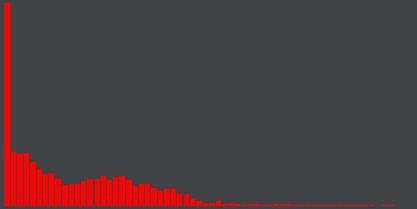
\includegraphics[width=0.31\linewidth]{histogram/histogram-boiler-groundtruth.png}}}
	\caption{Histograms of different streams of the \emph{boiler} data set at 0.08 bps. The
        {\em by level}, {\em by wavelet norm}, and {\em by signature}~\pavol{elsewhere histogram signature} streams
        produce histograms that have similar shape to the {\em groundtruth} histogram with most of the peaks and valleys
        preserved. In contrast, even though the {\em by bit plane} stream has similar mass distribution, it has one spurious
        peak that is not present in the {\em groundtruth} histogram.
        \pavol{are all those histograms normalized? why is there no greedy histogram?}}
	\label{fig:histograms-boiler}
\end{figure}

\pavol{summarize subsection}
In summary, we have evaluated six data sets, for each using different histogram streams, and
compared results with respect to the histogram intersection error and the visual differences. Interestingly, the
order of streams differs from all the other queries, where {\em by level} stream performed poorly, but for
histograms it outperforms both {\em by magnitude} and {\em by bit plane} streams.
The idea of signature works for histograms as well, and could be employed as a practical streaming
format, where the sender would first send the signature to the receiver at small cost (few integer
values). However, {\em by wavelet norm} stream has similar performance and does not require any extra
data transfered (such as signature), and thus we conclude that from
considered streams it has best properties.

% \begin{figure}
% 	\centering
% 	\subcaptionbox{\emph{histogram-optimized}}
% 	{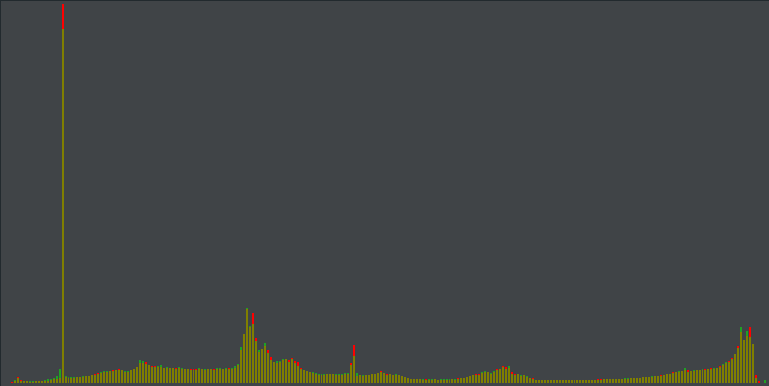
\includegraphics[width=0.48\linewidth]{img/histogram/histogram-signature.png}}
% 	\subcaptionbox{\emph{rmse-optimized}}
% 	{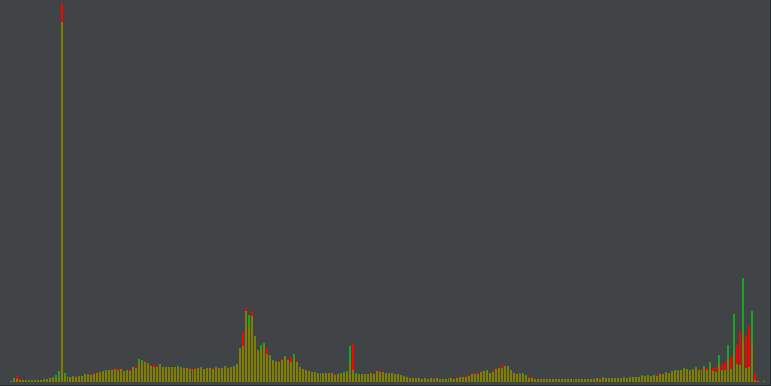
\includegraphics[width=0.48\linewidth]{img/histogram/histogram-by-wavelet-norm.png}}
% 	\caption{euler's histograms at 0.18 bps. The groundtruth histogram is rendered in red, while the
% 	reconstructed histogram is rendered in green. The dark yellow regions are where the two overlap.}
% 	\label{fig:histogram-comparison-low-bit-rate-slz}
% \end{figure}


\pavol{The visualization of the subbands is missing, but I think it was quite interesting and maybe we
should find a way to include it as it makes the discussion more interesting.}
%The main difference between the \emph{histogram-optimized} and the \emph{rmse-optimized} streams is
%that \emph{histogram-optimized} favors low-ordered bits of coarse-level coefficients, while,
%\emph{rmse-optimized} relatively favors high-ordered bits of fine-level coefficients. This is
%evident in Figure \ref{fig:histogram-signature-comparison} (b and d): for
%\emph{histogram-optimized}, the bright blue cells extend more toward the right (lower-ordered bit
%planes) and less toward the bottom (finer resolution levels). The histogram experiments in this
%Section are performed with 256 bins, but this fact holds for a wide range of number of bins. Figures
%\ref{fig:histogram-signature-comparison} (a, b, c) show that varying the number of bins from 128 to
%512 only affects the relative ordering among the low-ordered bits on very fine resolution levels
%(the dark blue cells at the bottom right of the signature). These are bits that come at the end of a
%stream, and thus matter little to the data quality. 

%The streams in Figure \ref{fig:histogram-comparison-low-bit-rate} (b, d, f, h) are truncated where
%the EMD errors of the \emph{histogram-optimized} streams are negligible, suggesting that it is often
%possible to achieve near lossless histograms with just 1 bit per sample. The boiler data set is a
%peculiar case, where the \emph{histogram-optimized} stream outperforms the rest of the streams by a
%large margin in the second half of the bit rate range. Looking at the precision maps (defined in
%Section [REF]) for the \emph{histogram-optimized} stream, as well as its reconstructed histogram
%(Figure \ref{fig:precision-map-histogram}, (a)), we see that the bit distribution is heavily
%concentrated in regions corresponding to one particular histogram bin that contains vastly more
%samples than other bins do. This situtation happens when there are many samples having essentially
%the same value but they are distributed irregularly in space (otherwise they would form constant
%regions which would be captured very well with just a few precision bits of wavelet coefficients --
%this is the case for the flame data set). In this case a stream needs to be more spatially adaptive
%to resolve well the histogram bin with the most samples, and among the tested streams, only
%\emph{histogram-optimized} is spatially adaptive to EMD (\emph{rmse-optimized} is spatially
%adaptive, but to RMSE, and the other two streams are data-independent).

% \begin{figure}[h]
% 	\centering
% 	\subcaptionbox{}
% 	{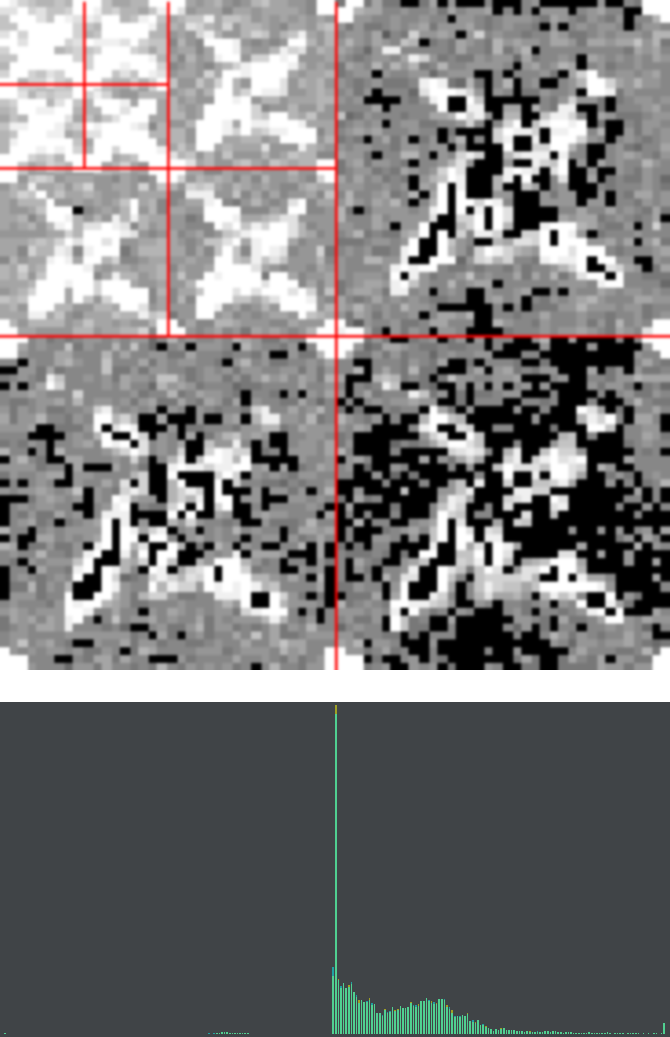
\includegraphics[width=0.24\linewidth]{img/histogram/boiler/prec-histogram_resize-vert.png}}
% 	\subcaptionbox{}
% 	{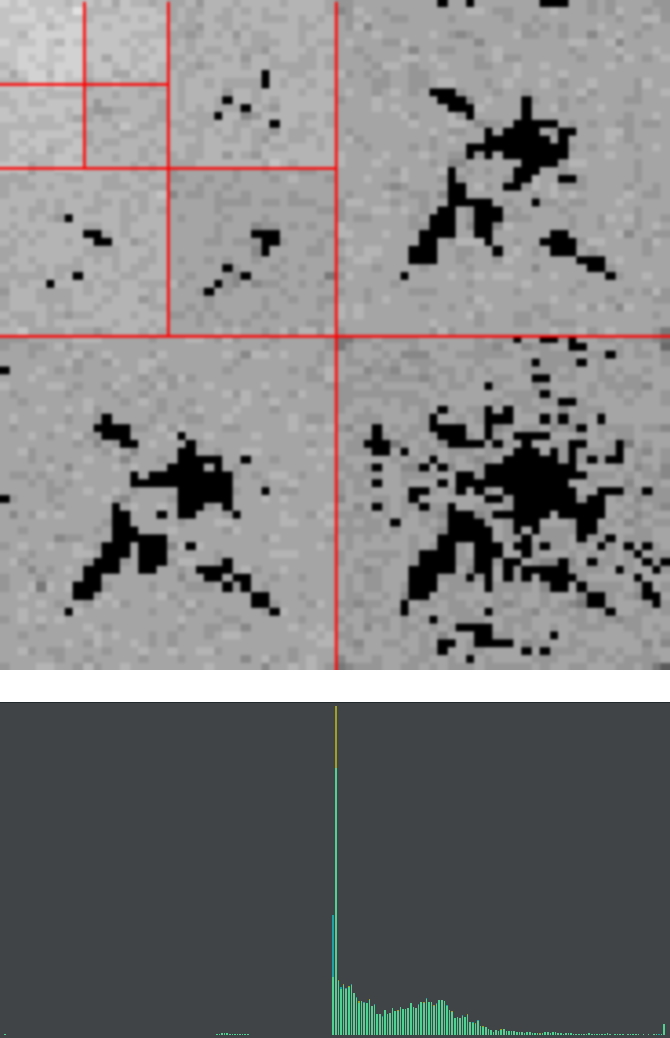
\includegraphics[width=0.24\linewidth]{img/histogram/boiler/prec-rmse_resize-vert.png}}
% 	\subcaptionbox{}
% 	{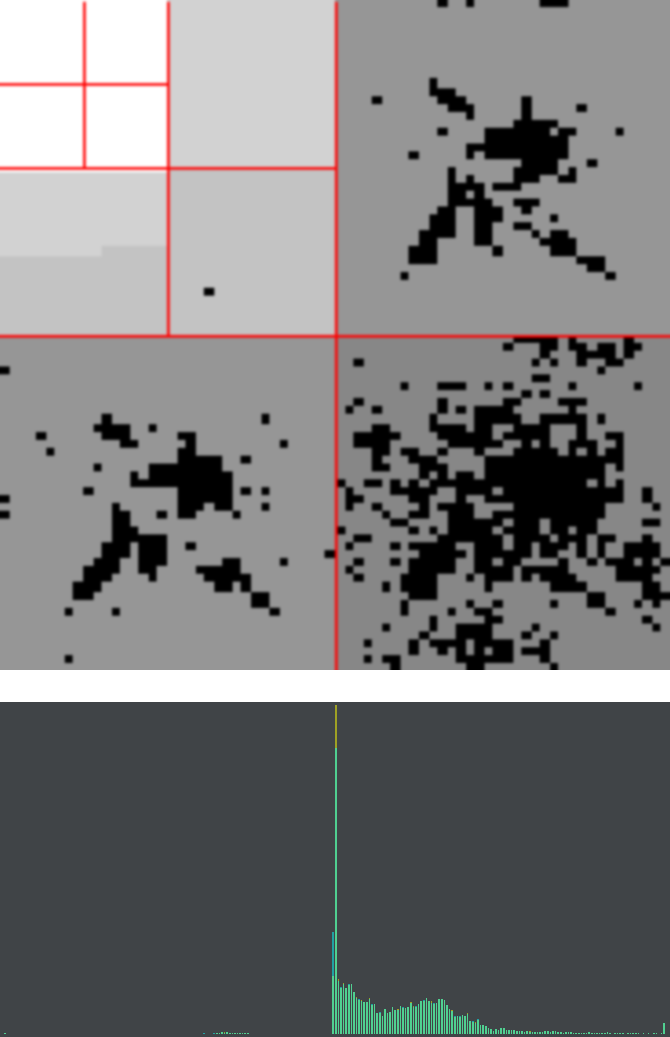
\includegraphics[width=0.24\linewidth]{img/histogram/boiler/prec-signature_resize-vert.png}}
% 	\subcaptionbox{}
% 	{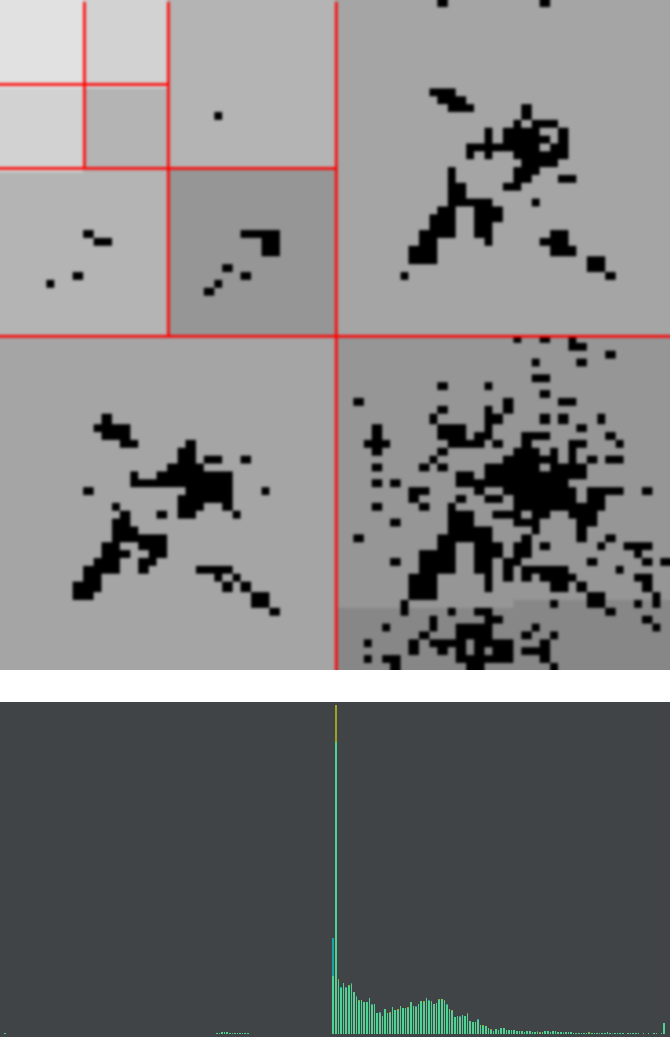
\includegraphics[width=0.24\linewidth]{img/histogram/boiler/prec-wavenorm_resize-vert.png}}
% 	\caption{(top) Precision distribution of wavelet coefficients, and (bottom) reconstructed
% 	histograms, for \emph{histogram-optimized}, \emph{rmse-optimized}, \emph{by wavelet norm}, and
% 	\emph{histogram signature} streams, at 6.47 bits per sample, without leading zero bits.}
% 	\label{fig:precision-map-histogram}
% \end{figure}

\duong{Discuss the case of not using compression, where the signature plays a more important role.}

%In this section we have shown that histogram computation requires a different ordering of bits than
%reconstructing the function itself. We have also proposed a practical heuristic, based on stream
%signatures, to capture the main characteristics of this ordering. In practice, the histogram
%signature can be pre-computed once and stored on disk. A signature's size is negligible (170
%integers in 2D and 374 integers in 3D in the case of four wavelet levels in each dimension), and can
%also be further compressed. Therefore it can be transmitted first, and the receiver of the data can
%ultilize the signature to smartly query the bits so as to reconstruct the data's histogram with as
%few bits as possible.
%%% Local Variables:
%%% mode: latex
%%% TeX-master: "template"
%%% End:
